\pagebreak
\subsection{Other critirea of measurability for Lebesgue measure}
As we remember, \hyperref[def:measurable]{the definition
of a measurable set} is difficult to check. Thus, we would like to have
better critirea.
\begin{theorem}
    $E \subset \mathbb{R}$ is Lebesgue measurable if and only if one of the following holds:
    \begin{enumerate}
        \item {
            For every $\varepsilon > 0$ there exists an open set $O$, such that
            $E \subset O$ and $m^*(O \setminus E) < \varepsilon$.
        }
        \item {
            There exists a $G_\delta$-set $G$, such that $E \subset G$ 
            and $m^*(G \setminus E) = 0$.

            (A $G_\delta$-set is a countable intersection of open sets.)
        }
        \item {
            For every $\varepsilon > 0$ there exists a closed set $F$, such that
            $F \subset E$ and $m^*(E \setminus F) < \varepsilon$.
        }
        \item {
            There exists a $F_\sigma$-set $F$, such that $F \subset E$
            and $m^*(E \setminus F) = 0$.

            (A $F_\delta$-set is a countable union of closed sets.)
        }
    \end{enumerate}
\end{theorem}
\begin{proof}
    \mbox{}
    \begin{itemize}
        \item {
            $E$ is measurable $\implies$ 1.

            If $m^*(E) < \infty$, then from the definition of $m^*$
            we can find $O$ --- a finite union of open intervals, such that
            $m^*(O) < m^*(E) + \varepsilon$. Since $O$ is an open set, it's
            measurable (as we proved \hyperref[the:openMeasurable]{earlier}).
            Therefore, both $E$ and $O$ are measurable, thus
            \[ \varepsilon > m^*(O) - m^*(E) \overset{E, O \in \mathcal{M}}{=} m^*(O \setminus E) \]

            If $m^*(E) = \infty$, let's split the set $E$ into a countable number of sets with
            finite measure. For example, by splitting the real line into 
            segments of length 1. So,
            $E = \cup_1^\infty E_k$, where $m^*(E_k) < \infty$.
            Then let's use geometrically decreasing $\varepsilon$'s for the covers of each
            $E_k$: $\varepsilon / 2$ for $E_1$, $\varepsilon / 4$ for $E_2$, and so on.
            When we sum up the inequalities, the fractions will sum up to $\varepsilon$.
            So, we obtained our $O$, now continue like in the previous case.
            \begin{definition}
                A measure $\mu$ on $X$ is called 
                \textit{$\sigma$-finite}, if $X = \cup_1^\infty X_k$ and
                $\mu(X_k) < \infty$ for all $k$. 
                
                In words:
                if there exists a subdivision of $X$ into a countable number
                of set of finite measure.
            \end{definition}
        }
        \item {
            $1 \implies 2$.

            From $1$, $\forall k \in \mathbb{N},\ \exists O_k$ ---
            open, such that $E \subset O_k$ and
            $m^*(O_k \setminus E) < \frac{1}{k}$.
            Now let's take
            \[
                G \coloneqq \bigcap_1^\infty O_k \implies
                \forall k:\ m^*(G \setminus E) \le m^*(O_k \setminus E) < \frac{1}{k}
                \implies m^*(G \setminus E) = 0
            \]
        }
        \item {
            $2 \implies E$ is measurable.

            $G$ is a $G_\delta$-set. As a countable intersection of open sets,
            it's in Borel $\sigma$-algebra, and thus is Lebesgue-measurable.
            $m^*(G \setminus E) = 0$, then $G \setminus E$ is Lebesgue-measurable,
            then $E = G \setminus (G \setminus E)$ is measurable as
            a difference of two measurable sets.
        }
        \item {
            $3 \Longleftrightarrow 1,\ 4 \Longleftrightarrow 2$.

            If we assume that 3 holds for $E$, then, if we take $O = \overline{F}$,
            1 will hold for $\overline{E}$.
            Therefore, $\overline{E}$ is measurable, then $E$ is measurable
            (as $\mathcal{M}$ is a $\sigma$-algebra).

            If 1 holds for $E$, then $E$ is measurable, then $\overline{E}$ is measurable, then 1 holds for 
            $\overline{E}$. Now take $F = \overline{O}$, therefore, 3 holds for $E$.

            \begin{figure*}[h]
                \centering
                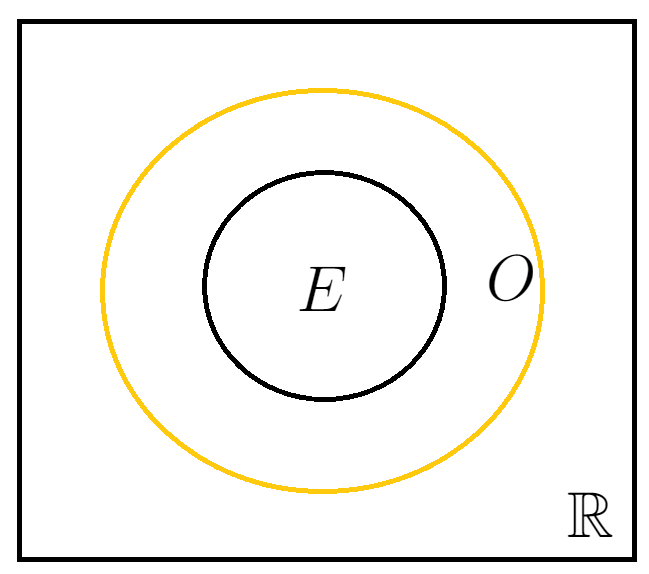
\includegraphics[width=0.3\textwidth]{e_o_r}
            \end{figure*}

            In the same way, 2 and 4 are equivalent as well.
        }
    \end{itemize}
\end{proof}

\begin{theorem}
    For every $E \in \mathcal{M}$ with $m(E) < \infty$ and for every
    $\varepsilon < \infty$ there exists an infinite disjoint collection of open intervals
    $\{I_k\}_1^n$, such that $O = \cup_{k=1}^n I_k$ and $m(E \triangle O) < \varepsilon$.

    (Here $\triangle$ is the symmetric difference of two sets).
\end{theorem}
\begin{proof}
    From part 1 of the previous theorem,
    we can take such an open set $U$, that $E \subset U$ and $m(U \setminus E) < \varepsilon / 2$. 
    
    As we proved \hyperref[prop:bIsSmallestSigmaAlgebra]{earlier}, 
    we can represent $U$ as a countable union of disjoint open intervals $I_k$. Then:
    \[
        \forall n: \bigcup_1^n I_k \subset U \implies \forall n:
        \sum_1^n m(I_k) \le m(U) < \infty
    \]
    Now take $n$, such that $\sum_{n+1}^\infty m(I_k) < \varepsilon / 2$, and put
    $O \coloneqq \cup_{k=1}^n I_k$.
    Then $m(O \setminus E) < \varepsilon / 2$ and $m(E \setminus O) < \varepsilon / 2$,
    therefore, the measure of the symmetric difference is less that $\varepsilon$.
\end{proof}

\subsection{TBA}

Questions:
\begin{enumerate}
    \item {
        If $m(A) = 0$, is $A$ countable?
    }
    \item {
        We know that $\mathcal{B} \subset \mathcal{M}$. Is this inclusion proper?
    }
\end{enumerate}

\begin{definition}[Cantor set]
    Let's take $[0, 1]$, split it into three parts and remove the middle part.
    Then continue such process.
    The \textit{Cantor set} is the set $C \coloneqq \cap_0^\infty C_k$.
\end{definition}

\begin{figure*}[h]
    \centering
    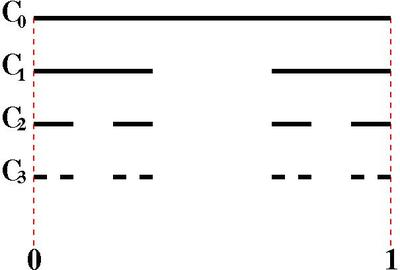
\includegraphics[width=0.3\textwidth]{cantor_set}
    \caption*{Cantor set illustration from \href{http://tasks.illustrativemathematics.org/content-standards/tasks/929}{here.}}
\end{figure*}

\begin{remark}
    Its length is zero as $(2/3)^\infty = 0$. But it's uncountable,
    because if we have a sequence of zeros and ones, we can traverse 
    down-left on 0 and down-right on 1. The intersection of the corresponding
    intervals will be a single point of $C$. So, there's a bijection between
    $C$ and $\{0, 1\}^\mathbb{N}$, therefore, $C$ is indeed uncountable. 
\end{remark}
